\chapter{Монады в Yesod}\label{chap:yesod_monads}

Как вы уже увидели, в этой книге появлялось несколько монад:
\lstinline'Handler', \lstinline'Widget' и~\lstinline'YesodDB' (для~Persistent).
Как и всякая монада, каждая из них предоставляет некоторую специфическую
функциональность: \lstinline'Handler' предоставляет доступ к запросу и позволяет
отправлять ответы, \lstinline'Widget' содержит HTML, CSS и Javascript, а
\lstinline'YesodDB' позволяет делать запросы к базе данных. В терминах
Model-View-Controller~(MVC), мы могли бы рассматривать \lstinline'YesodDB' как
модель, \lstinline'Widget'~--- как представление, а~\lstinline'Handler'~--- как
контроллер.

До сих пор у нас были представлены очень простые способы использования этих
монад: основной обработчик работает в монаде \lstinline'Handler', используя
\lstinline'runDB' для выполнения запроса~\lstinline'YesodDB' и
\lstinline'defaultLayout' для возврата~\lstinline'Widget', который, в свою
очередь, был создан вызовом~\lstinline'toWidget'.

Тем не менее, если у нас будет глубокое понимание этих типов, мы сможем достичь
более интересных результатов.

\section{Трансформаторы монад}
\hfill \begin{minipage}[h]{0.45\textwidth}
    \small
    Монады, они как луковицы. Монады \emph{не как} пирожные.
    \begin{flushright}
        \emph{Вроде бы Шрек}
    \end{flushright}
\end{minipage}
\vspace{2em}

Прежде чем мы углубимся в монады Yesod, мы должны немного понимать
трансформаторы монад.  (Если вы уже знаете о трансформаторах монад всё, вы,
скорее всего, можете пропустить этот раздел.) Различные монады предоставляют
различную функциональность: \lstinline'Reader' предоставляет доступ только для
чтения к некоторым данных по всему вычислению, \lstinline'Error' позволяет
обрывать вычисления, и так далее.

Часто, однако, хотелось бы иметь возможность комбинировать функциональность
некоторых из этих монад. В конце концов, почему бы не иметь вычисление с
доступом только для чтения к некоторым параметрам настройки, которое в любой
момент могло бы прерваться с ошибкой? Одним из подходов к решению могло бы стать
написание новой монады, например \lstinline'ReaderError', но это имеет очевидный
недостаток экспоненциальной сложности: потребуется писать новую монаду для
каждой возможной комбинации.

Вместо этого мы используем трансформаторы монад. Вместе с \lstinline'Reader', у
нас есть \lstinline'ReaderT', который добавляет функциональность
\lstinline'Reader' к любой другой монаде. Таким образом, мы могли бы представить
\lstinline'ReaderError' так (концептуально):
\begin{lstlisting}
type ReaderError = ReaderT Error
\end{lstlisting}

Чтобы получить доступ к параметру настройки, мы можем использовать
функцию~\lstinline'ask'. А что насчёт обрывания вычисления? Мы бы хотели вызвать
\lstinline'throwError', но это не вполне будет работать. Вместо этого мы должны
использовать \lstinline'lift', чтобы втянуть наш вызов в монаду на уровень
выше. Другими словами:
\begin{lstlisting}
throwError :: errValue -> Error
lift . throwError :: errValue -> ReaderT Error
\end{lstlisting}

Сейчас вы должны уловить несколько идей:
\begin{itemize}
    \item  Трансформатор может быть использован для добавления функциональных
        возможностей к существующим монадам.
    \item  Трансформатор должен всегда обёртываться вокруг существующей монады.
    \item  Функциональные возможности получившейся монады будут зависеть не
        только от трансформатора монады, но и от монады, обёрнутой внутри.
\end{itemize}

Отличный пример последнего утверждения~--- это монада \lstinline'IO'. Независимо
от того, сколько слоёв трансформаторов у вас есть вокруг \lstinline'IO', там всё
ещё есть ядро \lstinline'IO', то есть вы можете выполнять ввод/вывод в любом из
этих стеков трансформаторов монад. Вы будете часто видеть код, который выглядит
как \lstinline'liftIO $ putStrLn "Привет вам!"'.

\section{Три трансформатора}
Мы уже обсуждали два из наших трансформаторов ранее: \lstinline'Handler'
и~\lstinline'Widget'. Напомним два особых факта про них:
\begin{itemize}
    \item  Для упрощения сообщений об ошибках они не являются фактическими
        трансформаторами. Вместо этого, они объявлены как \lstinline'newtype' с
        жёстко заданной внутренней монадой.  Именно поэтому Yesod предоставляет
        специальную функцию \lstinline'lift', которая работает для
        \lstinline'Handler' и~\lstinline'Widget'.
    \item  На самом деле у них есть дополнительные параметры для типов подсайта
        и основного сайта. В результате, библиотеки Yesod предоставляют
        \lstinline'GHandler sub master a' и \lstinline'GWidget sub master a', а
        каждый сайт получает пару синонимов типов
        \lstinline'type Handler = GHandler MyApp MyApp'
        и~\lstinline'type Widget = GWidget MyApp MyApp ()'.
\end{itemize}

В пакете
\footnotehref{http://hackage.haskell.org/package/persistent}{persistent}, есть
класс типов~\lstinline'PersistStore'. Этот класс типов определяет все
примитивные операции, которые можно выполнять с базой данных, например,
\lstinline'get'. Этот класс типов по существу выглядит как
\lstinline'class (Monad (b m)) => PersistStore b m'. Где \lstinline'b'
определяет сервер базы данных, а на самом деле является трансформатором монады,
а \lstinline'm' является внутренней монадой, которую \lstinline'b' оборачивает.
И SQL, и MongoDB имеют свои собственные экземпляры; в случае SQL, он выглядит
так:
\begin{lstlisting}
instance MonadBaseControl IO m => PersistBackend SqlPersist m
\end{lstlisting}

Это означает, что вы можете работать с базой данных SQL при любой базовой
монаде, до тех пор, пока эта монада поддерживает \lstinline'MonadBaseControl IO',
позволяющую правильно обрабатывать исключения на стеке монад. В общем,
это означает любой стек трансформаторов, построенный вокруг \lstinline'IO'
(кроме исключительных случаев, как \lstinline'ContT'). К счастью для нас, это
включает в себя как \lstinline'Handler' так и \lstinline'Widget'. Следовательно,
мы можем наслаивать наш Persistent трансформатор на \lstinline'Handler'
или~\lstinline'Widget'.

\begin{remark}
Это не всегда было так. Перед Yesod 0.10, Yesod был построен на базе пакета
\texttt{enumerators}, который не поддерживает \lstinline'MonadBaseControl'. В
Yesod 0.10, мы перешли к пакету
\href{http://hackage.haskell.org/package/conduit}{conduit}\footnotemark, который
значительно упрощает всё, что мы здесь обсуждаем.
\end{remark}
\footnotetext{\href{http://hackage.haskell.org/package/conduit}{\texttt{http://hackage.haskell.org/package/conduit}}}

Для того, чтобы упростить обращение к соответствующим Persistent
трансформаторам, пакет
\footnotehref{http://hackage.haskell.org/package/yesod-persistent}{yesod-persistent}
определяет ассоциированный тип~\lstinline'YesodPersistBackend'. Например, если у
нас есть сайт, который называется \lstinline'MyApp' и использует SQL, мы можем
определить что-то вроде
\lstinline'type instance YesodPersistBackend MyApp = SqlPersist'.

Когда мы захотим выполнить наши действия с базой данных, у нас будет
\lstinline'SqlPersist', обёрнутый вокруг \lstinline'Handler' или
\lstinline'Widget'. Так мы сможем использовать стандартные функции развёртки
Persistent (например, \lstinline'runSqlPool') для исполнения действия и возврата
в нормальный \lstinline'Handler/Widget'. Для автоматизации этого,
предоставляется функция \lstinline'runDB'. Суммируя всё это, мы теперь можем
исполнять действия с базой данных внутри наших обработчиков и виджетов.

Большую часть времени в коде Yesod, и особенно на протяжении предыдущих глав,
виджеты рассматривались как контейнеры, которые просто объединяют вместе HTML,
CSS и Javascript и не содержат действий. Но если вы посмотрите на последний
абзац ещё раз, вы поймёте, что это не обязательное требование. Поскольку
виджет~--- это трансформатор над обработчиком, всё, что вы делаете в
обработчике, может быть сделано в виджете, в том числе и операции с базой
данных. Всё, что вам нужно сделать,~--- это протянуть вызов, используя
\lstinline'lift'.

\section{Пример: навигационная панель на основе базы данных}
Давайте применим некоторые из новых знаний на практике. Мы хотим сделать виджет,
который генерирует свой вывод на основе содержимого базы данных. Ранее мы бы
загрузили данные в обработчике, а затем передали эти данные в виджет. Теперь же
загрузим данные в самом виджете. Это хорошо для модульности, так как этот виджет
может использоваться в любом обработчике по нашему желанию, без необходимости
передавать содержимое базы данных.

\includecode{13/navbar.hs}

В частности, обратите внимание на функцию \lstinline'existingLinks'. Заметьте,
всё, что нужно сделать,~--- это применить \lstinline'lift' к обычному действию с
базой данных. А в \lstinline'getRootR', мы трактуем \lstinline'existingLinks'
как обычный виджет без каких-либо специальных параметров вообще. На
рисунке представлен вывод этого приложения.

\begin{figure}[tbh]
  \centering
  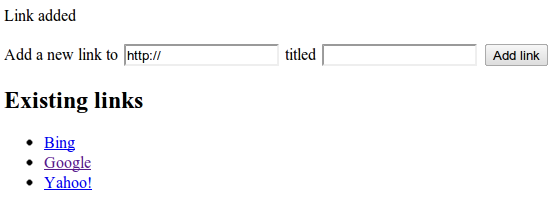
\includegraphics[scale=0.5]{13-yesods-monads-image-01.png}
  \caption{Скриншот панели навигации}
\end{figure}

\section{Пример: информация из запроса}
Таким же образом вы можете получить информацию из запроса внутри виджета. В
примере ниже мы определяем порядок сортировки списка на основе значения
параметра GET-запроса.

\includecode{13/request-information.hs}

Повторим, всё, что нужно сделать,~--- это протянуть функцию стандартную для
обработчика (в данном случае, \lstinline'runInputGet'), чтобы выполнить её в
нашем виджете.

\section{Выводы}
Если вы полностью пропустили эту главу, вы всё равно сможете с большой пользой
использовать Yesod. Преимущество понимания как взаимодействуют монады
Yesod~--- возможность производить более чистый и более модульный код. Способность
выполнять произвольные действия в \lstinline'Widget' может быть мощным инструментом, и
понимание того, как взаимодействуют \lstinline'Persistent' и ваш \lstinline'Handler' код,
может помочь вам сделать более обоснованные проектные решения в вашем приложении.
